
\documentclass[10pt,a4paper,twoside,openright,fleqn,%
               parskip=half,%
               BCOR=5mm,DIV=10,footinclude=false%
               numbers=noenddot,cleardoublepage=empty]{scrbook}

\usepackage[utf8]{inputenc} 
\usepackage{mathpazo} %-- use Palatino font
\usepackage{amsmath,amssymb,amsthm}
\usepackage[square]{natbib}
\usepackage{subcaption} 
\usepackage{xspace}
\usepackage[breaklinks=true,
            colorlinks=true,
            linktocpage=true,
            allcolors=colorforlinks]{hyperref} 
\usepackage[ruled,vlined,algochapter,linesnumbered]{algorithm2e}
\usepackage{calc}
\usepackage{ccicons} 
\usepackage{xspace} 
\usepackage{booktabs} 
\usepackage[english]{babel}  
\usepackage{listings}
\usepackage{scrhack} % ignore warnings about deprecated KOMA-Script
\usepackage[printonlyused,smaller,withpage]{acronym}
\usepackage[usenames,dvipsnames]{xcolor}
\usepackage{graphicx}
\usepackage{pdfpages}
\usepackage{todonotes}






\newcommand{\myName}{Jos Feenstra}
\newcommand{\myTitle}{Geofront: Library portability in a browser based visual programming language for geo-computation}

\newcommand{\myGroup}{3D geoinformation group}
\def\myGroupLogo{figs/tud-3dgeoinfo-black.png}
\newcommand{\myUni}{Delft University of Technology}

\newcommand{\myGraduationYear}{2022}
\newcommand{\myGraduationMonth}{June}

\newcommand{\mySupervisorOne}{Ir.\ Stelios Vitalis}
\newcommand{\mySupervisorTwo}{Dr.\ Ken Arroyo Ohori}
\newcommand{\mySupervisorThree}{Dr.\ Giorgio Agugiaro}
\newcommand{\myCoreader}{Dr.\ Hugo Ledoux}

%-- for names for \autoref commands
\def\chapterautorefname{Chapter}
\def\sectionautorefname{Section}
\def\subsectionautorefname{Section}
\def\subsubsectionautorefname{Section}
\def\algorithmautorefname{Algorithm}

% a way to make images fit the paper
% https://tex.stackexchange.com/questions/86350/includegraphics-maximum-width
\def\maxwidth{460pt} 


%-- for pdf metadata
\hypersetup{pdfauthor={\myName}}
\hypersetup{pdfkeywords={thesis, geomatics, TU Delft}}
\hypersetup{pdfsubject={A thesis submitted to the Delft University of Technology in partial fulfillment of the requirements for the degree of Master of Science in Geomatics}}
\hypersetup{pdftitle={\myTitle}}

%-- handy shortcuts
\newcommand{\ie}{i.e.}
\newcommand{\eg}{e.g.}
\newcommand{\reffig}[1]{Figure~\ref{#1}}
\newcommand{\refsec}[1]{Section~\ref{#1}}
\newcommand{\refchap}[1]{Chapter~\ref{#1}}

% [JF]: added a command to prettify this dodgy syntax. m stands for monospace
\newcommand{\m}[1]{\texttt{#1}}

%-- colours for the hyperlinks
\definecolor{colorforlinks}{RGB}{27, 60, 131}

\lstdefinestyle{note}
{
    breaklines=true, 
    basicstyle=\footnotesize,
    keywordstyle=\color{blue},
    commentstyle=\color[rgb]{0.13,0.54,0.13},
    backgroundcolor=\color{cyan!10},
}
\lstnewenvironment{note}
{\lstset{style=note}}
{}

% I keep changing the styling of geofront, so lets put them here
\newcommand{\geofront}{Geofront}

% I keep changing research questions, so lets put them here
% \newcommand{\myMainRQ}{\textit{How to design and implement a web-based vpl for geo-computation which supports running existing geo-computation libraries in a web browser?}}
\newcommand{\myMainRQ}{\textit{How can native geocomputation libraries be \emph{compiled}, \emph{loaded}, and \emph{utilized} within a browser-based dataflow-VPL?}}

\newcommand{\mySubRQOneTitle}{Representation} % previously: facilitation
% \newcommand{\mySubRQOne}{\textit{To what extent is a browser-based application able to facilitate a generic 3D geometry vpl?}}
\newcommand{\mySubRQOne}{\textit{How to implement a browser-based dataflow-vpl for processing 3D geometry?}}

% \newcommand{\mySubRQOne}{\textit{How to implement a visual programming environment in a browser which able to facilitate geo-computation?}}
\newcommand{\mySubRQTwoTitle}{Compilation}
\newcommand{\mySubRQTwo}{\textit{How can geocomputation libraries written in system-level languages be \textbf{compiled} for web consumption?}}
\newcommand{\mySubRQThreeTitle}{Loading}
\newcommand{\mySubRQThree}{\textit{To what extent can a web-consumable library be \textbf{loaded} into a web-vpl without explicit configuration?}}
\newcommand{\mySubRQFourTitle}{Utilization}
% \newcommand{\mySubRQFour}{\textit{What are the advantages and disadvantages of \textbf{using} an existing geoprocessing library through a geo-web-vpl, as opposed to native utilization of said library?}}
\newcommand{\mySubRQFour}{\textit{How can a 'geo-web-vpl' be \textbf{used} to create geodata pipelines?}}








% ********************************************************************
% listings from arsclassica
% ********************************************************************

\let\orgtheindex\theindex
\let\orgendtheindex\endtheindex
\def\theindex{%
	\def\twocolumn{\begin{multicols}{2}}%
	\def\onecolumn{}%
	\clearpage
	\orgtheindex
}
\def\endtheindex{%
	\end{multicols}%
	\orgendtheindex
}

\makeindex

% ********************************************************************
% listings
% ********************************************************************

\definecolor{lightergray}{gray}{0.99}

\lstset{language=[LaTeX]Tex,
    keywordstyle=\color{RoyalBlue},
    basicstyle=\normalfont\ttfamily,
    commentstyle=\color{Emerald}\ttfamily,
    stringstyle=\rmfamily,
    numbers=none,
    numberstyle=\scriptsize,
    stepnumber=5,
    numbersep=8pt,
    showstringspaces=false,
    breaklines=true,
    frameround=ftff,
    frame=lines,
    backgroundcolor=\color{lightergray}
} 

\lstset{morekeywords=%
        {function, f32, i32},
        commentstyle=\color{Emerald}\ttfamily,%
        frame=lines}

\lstset{basicstyle=\normalfont\ttfamily}
\lstset{flexiblecolumns=true}
\lstset{moredelim={[is][\normalfont\itshape]{/*}{*/}}}
\lstset{basicstyle=\normalfont\ttfamily}
\lstset{flexiblecolumns=false}
\lstset{moredelim={[is][\ttfamily]{!?}{?!}}} 
\lstset{escapeinside={£*}{*£}}
\lstset{firstnumber=last}
\lstset{moredelim={[is][\ttfamily]{!?}{?!}}}

\DeclareRobustCommand*{\pacchetto}[1]{{\normalfont\ttfamily#1}%
\index{Pacchetto!#1@\texttt{#1}}%
\index{#1@\texttt{#1}}}

\DeclareRobustCommand*{\bibtex}{\textsc{Bib}\TeX%
\index{bibtex@\textsc{Bib}\protect\TeX}%
}

\DeclareRobustCommand*{\amseuler}{\protect\AmS{} Euler%
\index{AmS Euler@\protect\AmS~Euler}%
\index{Font!AmS Euler@\protect\AmS~Euler}}

\lstnewenvironment{code}% 
{\setkeys{lst}{columns=fullflexible,keepspaces=true}%
\lstset{basicstyle=\small\ttfamily}%
}{}

\lstset{extendedchars} 
\lstnewenvironment{sidebyside}{% 
    \global\let\lst@intname\@empty 
    \setbox\z@=\hbox\bgroup 
    \setkeys{lst}{columns=fullflexible,% 
    linewidth=0.45\linewidth,keepspaces=true,%
    breaklines=true,% 
    breakindent=0pt,%
    boxpos=t,%
    basicstyle=\small\ttfamily
}% 
    \lst@BeginAlsoWriteFile{\jobname.tmp}% 
}{% 
    \lst@EndWriteFile\egroup 
        \begin{center}% 
            \begin{minipage}{0.45\linewidth}% 
                \hbox to\linewidth{\box\z@\hss} 
            \end{minipage}% 
            \qquad 
            \begin{minipage}{0.45\linewidth}%
            \setkeys{lst}{frame=none}% 
                \leavevmode \catcode`\^^M=5\relax 
                \small\input{\jobname.tmp}% 
            \end{minipage}% 
        \end{center}% 
} 

\lstset{numbers=left,
    numberstyle=\scriptsize,
    stepnumber=1,
    numbersep=8pt
}   

\setcapindent{1em} %-- for captions of Figures
% \setcounter{tocdepth}{\sectiontocdepth}

\subject{MSc thesis in Geomatics}
\title{\myTitle}
\author{\myName}
\date{\myGraduationMonth\xspace\myGraduationYear}
\publishers{A thesis submitted to the Delft University of Technology in partial fulfillment of the requirements for the degree of Master of Science in Geomatics}

\begin{document}


%******************************************************************
% Frontmatter
%******************************************************************
\frontmatter

%******************************************************************
% The cover page 
% (it needs to be manually edited and exported as a PDF)
% (see folder README.txt in folder 'cover')
% (I would not include it for the version you put in the repository)
%******************************************************************

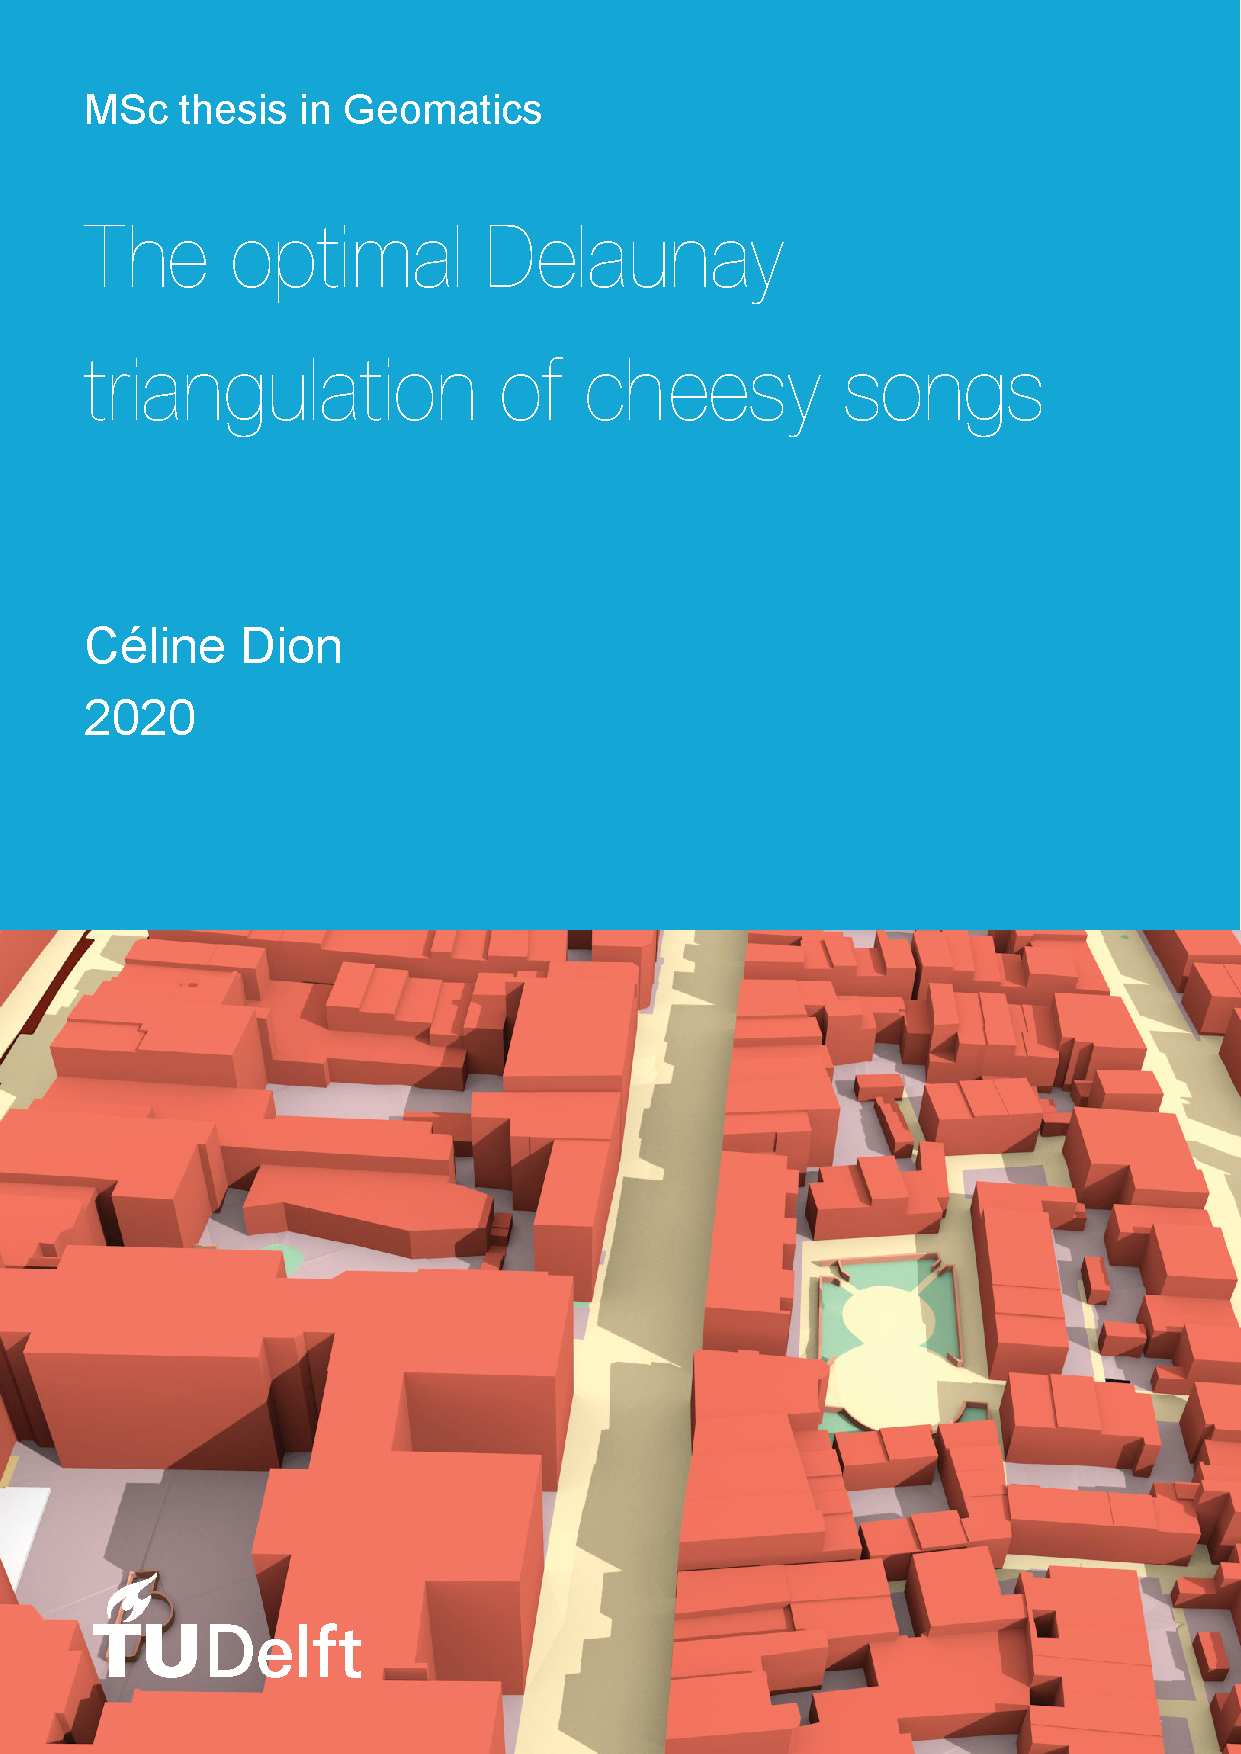
\includepdf{cover/cover_front.pdf}
\cleardoublepage

\maketitle[3]

% \clearpage
%!TEX root = ../thesis.tex

\thispagestyle{empty}

\hfill
\vfill

\noindent\myName: \textit{\myTitle} (\myGraduationYear)\\
\ccby\xspace This work is licensed under a Creative Commons Attribution 4.0 International License. To view a copy of this license, visit \url{http://creativecommons.org/licenses/by/4.0/}.

\vspace{3em}


\vspace{3em}

\noindent{} The work in this thesis was carried out in the:\\

\begin{tabular}{ll}
\parbox{0.3\textwidth}{\includegraphics[width=\linewidth]{\myGroupLogo}}
&
\parbox{0.7\textwidth}
{
  \myGroup\\
  \myUni\\
}       
\end{tabular}

\vspace{3em}
\noindent
\begin{tabular}{ll}
Supervisors:  &  \mySupervisorOne \\
              &  \mySupervisorTwo \\
Co-reader:    &  \myCoreader\\
\end{tabular}


\cleardoublepage
\chapter*{Abstract}

X is an essential part of any ...

The problem ...

The goal of this study is to

This study presents and prototypes a novel method which allows \ac{GIS} practitioners without a background in software development, to access the full potential of core transformation and analysis capabilities found in native \ac{GIS} libraries.

% That is based on visual programming, and static web applications. 


% The study attempts to meet this goal by designing and implementing a 
novel method based on the fields of visual programming, and static web applications. 

% The prior works on static geo-web applications and \ac{GIS} \ac{VPL}s indicate that a strong theoretical framework is in place.
% But, and this is especially evident in the prior studies regarding Browser-based geocomputation, the practical implementation of these theories were only partially successful, and limited in scope. 
% This necessitates a practical approach in response. 

A Prototype VPL was developed to host the functionalities of \ac{GIS} libraries from within an application, and in a composable manner. Additionally, it is used to connect these libraries to various \ac{GUI} features. 
The format of web application is used to allow this prototype to be directly accessible to end users without installation or configuration. 
% Geodata used within the application is also exclusively statically hosted geodata, or user-submitted data. 
This prototype is statically hosted, to minimize operational costs, and is equipped with WebAssembly, so that libraries written in native languages can be used without resorting to active backend web services. 
Finally, as this prototype is intended for \ac{GIS} usage, both scalability to handle sizable datasets, and rich \ac{GUI} support (3D viewers, file inputs, sliders, text boxes, graphs), are primary design considerations and assessment criteria.

Using this, ...

This method turned out to indeed provide solve

The significance of this method lies herein that it ...


% This method is thereafter used to load various \ac{GIS} libraries, and used in demo applications, after which an assessment can be made on its quality and the extend of its achieved functionalities. 
% The study concludes by addressing if the method meets the overarching goal.


% Geocomputation is a cornerstone of GIS \& modern mapping needs.
% While the last decades have seen major advancements, writing a geocomputational pipeline remains a complex, non-trivial exercise. 
% Performing geocomputations by utilizing a visual programming language (VPL) within a web browser is a novel development which seeks to simplify this process, allowing more people to write these types of pipelines more successfully.
% It would, in theory, allow end-users to author geocomputation pipelines, without the need of a software development background, and without the need to install software.
% utilizing a dataflow model.
% This model is the standard within VPLs dealing with geometry processing, and contains many advantages in terms of performance and reliability.

% In this context, the portability of existing geocomputation libraries is a common problem.
% This is often addressed by maintaining duplicate JavaScript alternatives to libraries such as GDAL, PROJ, and GEOS, complicating innovation.  

% This study seeks to improve the state of browser-based geocomputation VPLs by attempting to bring industry-standard geo-libraries to these environments. 
% The study poses that this can only be done if native geocomputation libraries can be \emph{compiled} to WebAssembly, \emph{loaded} into a VPL, and \emph{utilized} in a browser-based dataflow-VPL format.
% Discovering if and how these steps can be performed is the central question of this study. 
% % This study seeks to improve the state of web-based geocomputation VPLs 
% % by discovering if the library portability problem can be overcome, and if so, how.

% This question is answered by testing a possible solution.
% A proof of concept web-based VPL is designed, implemented and evaluated, which makes use of a novel plugin system, as well as a directed, acyclic graph-based data model \& interface.

% Using this proof of concept, the study was able to demonstrate that the web platform was sufficiently capable of representing a dataflow VPL capable of constructing geocomputation pipelines.
% The functional programming-properties of this dataflow VPL also makes geo-libraries sufficiently \emph{usable}, albeit with some well-known caveats of dataflow-VPLs, like the representation of conditionals and iteration.  

% The current methods of \emph{compiling} existing C++ geocomputation libraries to the web turned out to be insufficient for the purposes of this study.  
% This is due to the Emscripten compiler's focus on compiling full C++ applications instead of separate libraries. 
% Despite this, the study wás able to demonstrate how a novel method can be used to sufficiently \emph{compile} and \emph{load} multiple Rust-libraries for usage in the VPL, thanks to more feature-rich WebAssembly tools in the Rust ecosystem. 
% While Rusts geocomputation libraries are young, the study presents this method to either offer emscripten contributors a blueprint of a desired workflow, or to offer geocomputation library contributors a powerful use-case for the Rust language. 

% All in all, this means that either if the geocomputation libraries found in the Rust ecosystem mature, or if Emscripten's capabilities improve, then the code portability problem \& dataflow problem of existing web-based geocomputation VPLS can be solved. 


% \begin{note}

%     "make a simple narrative of what you did and what are the results."
%     "make it not be a very rough draft"
%     "6.2: deliver the things you promised."
%     "make it more formal: replace: "crucial", "by far" or "impressive""

%     Stelios Draft Comments
%     ======================
    
%     In general, I think it's going well. I think the intro is fine, although it can be improved. I like the conclusions quite a lot, tbh. You are giving proper and interesting answers to the raised questions. The rest is a bit of a very rough draft, as I see. So, some specific points:
    
%     TODO: Tone down stuff
%     -  It seems like you have placed several bits here and there that seem like either introduction or conclusions. I feel your enthusiasm and excitement in your writing, but I think you are bringing questions and answers in places were people would normally just expect a simple narrative of what you did and what are the results.
    
%     TODO: Write 6.2
%     -  Speaking of results, we are missing the experiments so please put this at your first priority. This is because it feels like you promise things that you do not deliver.
    
%     TODO: Find & Replace
%     -  In general, you are using some very bold statements and informal expressions. The latter is kinda okay, but the first one is very dangerous. I've noticed words like "crucial", "by far" or "impressive" which seem very biased and subjective, so better be avoided. You can still use them here and there (mostly in the conclusions), but I think you use them way  too much (again, I can see your enthusiasm).
    
%     TODO: Find & Replace 
%     -  Minor thing, but I think you have confused \citet with \citep. The first one is used when the citation is part of the sentence and the latter when it's at the end of a sentence (or in a parenthesis, anyway).
    
% \end{note}

% This might allow web based VPLs for geocomputation to be 
% Geodata computation is important.
% Geodata computation is difficult.
% geo-web-vpls could help, but have seen little research
% This study: design, implement, analyze a new prototype geo-web-vpl. 
% Design-> utilize existing, native libraries written in C++ \& Rust on the web, in the format of a vpl.

% results -> it works.

% -> study shows that interplay between textual and visual programming is possible


% \begin{note}
%  - Performance intensive: (Big data, O(n^2) problems) 
%  - Heterogenous data (type, quality, scale, criteria, crs) 
%  - Complex (geometric) operations (linalg, bundle adjustment, procedural modelling) 
% \end{note}

% All of this makes the process of geocomputation difficult. 


% The full flowchart runs client-side in a browser, and both end results and intermediate products can be inspected in a 3D viewer.

% GeoFront offers several functionalities such as the parametric creation of 2D and 3D primitives, triangulation, isocurve extraction, and more. 
% These functionalities can be expanded upon though a plugin system which utilizes the existing "Node Package Manager" infrastructure.
% Together with WebAssembly, this enables the utilization of industry standard geoprocessing libraries such as `CGAL`, `GDAL` and `PROJ`, and data parsing libraries such as `IFC.js` and `laz-rs`.



% Following the implementation, the project was tested by simulating use-case scenarios. 
% The tests demonstrate the feasibility of [...]
% At the same time some key parameters of [...] identified which if tuned properly they can optimize the performance, behavior and robustness of the geo-web-vpl.
% With the project being a prototype solution, the vpl is far from operational and there is certainly a lot of space for improvement regarding both components. 

% 1. Tryout (ACTUAL)
%    - A-la wapm WebAssembly Package Manager allows packages to be run from within the package-page itself. 
%   - Just meant to quickly try out some features.

% 2. Educational (ACTUAL)
%    - interactive educational tool
%    - (What does a delaunay triangulation look like? how does it behave? What happens if you lower the radius of inverse distance weighting ? )

% 3. Rapid-Prototyping (POSSIBLE)
%    - Setting up pipelines which can be consumed by cloud-based geoprocessing services. 
%    - Future work: export flowchart to a process which can be run natively or server side.

% 4. Publishing (POSSIBLE)
%    - Geotiff.io / ModelLab
%    - Web FME 
%    - Publish full web apps in and off themselves, making use of zero, one or multiple wasm-compiled libraries.  
%    - Future work: export to web-app (without flowchart)

% % Safesoft's FME, but web based \& open source 

% % CONCLUSION
% By creating geofront, this thesis was able to discover .............

% - The web is able to facilitate a visual proregramming language.

% - The web is able to be used for geoprocessing, albeit with some caveats
%   - TypedArrays,
%   - Geometric predicates 
%   - Rounding
%   - ETC.

% - Many of these things can be fixed with webassembly, but webassembly itself has other shortcomings
%   - Differences between Rust \& C++

% - reasonable performance 
%   (- great considering the platform)

% - would not be possible without these modern web features
%   - Web Assembly 
%   - Typed Array's 
%   - Web Workers
%   - Web Components,
%   - 2D Canvas API
%   - Web GL

% \todo{[JF]: I need to add more critical notes on promises of accessibility. Is a webapp truly accessible? Is a flowchart interactive, or does it hinder interactiveness? }

% I believe that such a web application can make geoprocessing more accessible to practitioners.
% This empowers users to create small geoprocessing demo's, and share these 
% With geofront, geoprocessing libraries can be loaded and used interactively. Users are also able to create and share flowcharts.
%%%%%%%%%%%%%%%%%%%%%%%%%%%%%%%%%%%%%%%%%%%%%%%%%%%%%%%%%%%%%%%%%%%%%%

% 


%%%%%



\begin{note}

  Lessons
  ==========
  
  - give yourself clear todo's per day. 
    Not too little, not too much.
    Upon completion, the day falls apart
  
  
  TODO
  ============
  
  high-level
  ----------
  
  [x] The intro / story needs to be altered 
      - stronger tie to Geo & web
      - VPL + Web
  
  [x] rewrite and balance research questions
  - [x] then trickle down the consequences of those changes throughout the thesis
  mid-level
  ---------
  
  [ ] TODO: rewrite abstract in accordance with new story

  [x] Deep dive in Hugo's comments, fix those aspects 
    - [x] sort acronyms
  
  [x] Add a stronger web-component in the introduction (presentation)
  [x] Add cloud native / cloud-based geodata component to the introduction  
  
  [ ] Cleanup Chapter 2 and 3.  
    - Some parts are still more relevant than other parts. 
    - Also, there are some things I say or use in chapter 4, 5, and 6, that were not properly explained in chapter 2. Examples of this are emscripten, or CGAL. 
    - However, a complete rewrite would be too much work.
    - Would love to hear your take on this.
  
  [ ] Make chapter 4 and 5 more streamlined 
    - I've noticed that I repeat myself quite often.
    - I think this is because I was not sure if I already said something relevant in the chapter before.
  
  [ ] Show your results more clearly, do the coding you have done justice
  
  [ ] finish chapter 6 properly 
    - Experiments: add a section on a use-case application, using potree + startin + geofront std + obj downloader
  
  [x] write stronger, more clear conclusions.
    - hmm, i think they are already quite clear. But again, this is to be reconsidered when the overall story of the thesis changes  
  
  low-level: thursday & friday
  -------------------

  - [ ] write 
  - [x] TODO: write Acknowledgements
  - [x] Add arsclassica template to the thesis
  - [x] Make the code snippets / listings work properly
  - [x] replace all code screenshot with proper listings
  - [ ] create all missing uml diagrams
  - [ ] add proper graphs for the data you've gathered 
  - [ ] Add all proper metadata to Zotero, for a nice bibliography
  - [ ] Fix all TODO graphics
  - [ ] Fix all acronyms,
  - [ ] Sort the acronyms at the end 
  - [ ] Make sure CiteT and citeP is properly used everywhere. No more raw 'et. al.' statments 
  - [ ] Capitalize all VPL / replace with acronyms
  - [ ] Sources need to be fixed (more data, check if I can do things like 'empscripten contributors')
  - [ ] Replace C++ into C / C++ everywhere, but especially the intro
  - [ ] appendix: software implementation & link to video
\end{note}


\chapter*{Acknowledgements}

\begin{itemize}
    \item Stelios
    \item Ken
    \item Martin, Current employer, GeoDelta 
    \item Sybren, Previous employer, Sfered
    \item Nadja
    \item Tim
    \item Friends \& Family
\end{itemize}

\ldots



 
\clearpage

\setcounter{tocdepth}{2}

\tableofcontents
\listoffigures
% \listoftables
% \listofalgorithms


\clearpage
\chapter*{Acronyms}

% thank you, vscode sort lines extension!
\begin{acronym}
    \acro{CDN}{Content Delivery Network}
    \acro{CGAL}{Computational Geometry Algorithms Library}
    \acro{CLI}{Command Line Interface}
    \acro{CRS}{Coordinate Reference System}
    \acro{DAG}{Directed Acyclic Graph}
    \acro{DEM}{Digital Elevation Model}
    \acro{DT}{Delaunay triangulation}
    \acro{DTM}{Digital Terrain Model}
    \acro{DSM}{Digital Surface Model}
    \acro{ETL}{Extract Transform Load}
    \acro{EUD}{End User Development}
    \acro{FOSS}{Free and Open Source Software}
    \acro{GDAL}{Geospatial Data Abstraction Library}
    \acro{geo-vpl}{geocomputation or geometry VPL}
    \acro{geocomputation}{Geospatial data computation}
    \acro{GEOS}{Geometry Engine Open Source}
    \acro{GIS}{Geographical Information Science}
    \acro{GUI}{Graphical User Interface}
    \acro{HTTP}{Hyper Text Transfer Protocol}
    \acro{IDE}{Integrated Development Environment}
    \acro{MVC}{Model View Controller}
    \acro{os}{operating system}
    \acro{OSGEO}{Open Source Geospatial Foundation}
    \acro{OGC}{Open Geospatial Consortium}
    \acro{TIN}{triangular irregular network}
    \acro{UI}{User Interface}
    \acro{UX}{User Experience}
    \acro{VD}{Voronoi diagram}
    \acro{VPL}{Visual Programming Language}
    \acro{W3C}{World Wide Web Consortium}
    \acro{wasm}{WebAssembly}
    \acro{WFS}{Web Feature Service}
    \acro{WMS}{Web Mapping Service}
    \acro{WPS}{Web Processing Service}
    % \acro{etl}{Extract Load Transform}
\end{acronym}


% WHY DOESNT THIS SHOW UP???
% https://tex.stackexchange.com/questions/557187/acronyms-in-a-table-environment-are-not-shown-in-the-list-of-acronyms


\cleardoublepage

%******************************************************************
% Mainmatter
%******************************************************************
\mainmatter

%!TEX root = ../thesis.tex
\chapter{Introduction}%
\label{chap:introduction}


This is a complete template for the MSc Geomatics thesis.
It contains all the parts that are required and is structured in such a way that most/all supervisors expect.
Observe that the MSc Geomatics at TU Delft has no formal requirements, how the document looks like (fonts, margins, headers, etc) is entirely up to you. 

We basically took the template \texttt{KOMA-Script scrbook}, added the front/back matters (cover page, copyright, abstract, etc.), and gave examples for the insertion of figures, tables and algorithms.

\emph{It is not an official template and it is not mandatory to use it.}

But we hope it will encourage everyone to use \LaTeX\ for writing their thesis, and we also hope that it will \emph{discourage} some from using Word.

If you run into mistakes/problems/issues, please report them on the GitHub page, and if you fix an error, then please submit a pull request. 

\url{https://github.com/tudelft3d/msc_geomatics_thesis_template}.


%%%
%
\section{How to get started with \LaTeX?}%
\label{sec:startlatex}



Follow the Overleaf's Learn LaTeX in 30min (\url{https://www.overleaf.com/learn/latex/Learn_LaTeX_in_30_minutes}) to start.

The only crucial thing missing from it is how to add references, for this we suggest you use \texttt{natbib} tutorial (\url{https://www.overleaf.com/learn/latex/Bibliography_management_with_natbib}).

%%%
%
\section{Cross-references}

The command \texttt{autoref} can be used for chapters, sections, subsections, figures, tables, etc.

\autoref{chap:introduction} is what you are currently reading, and its name is \nameref{chap:introduction}.
\autoref{sec:code} is about pseudo-code, and \autoref{sec:pdf} is about something else.
The next chapter (\nameref{chap:rw}), is on page~\pageref{chap:rw}.


%%%
%
\section{Figures}%
\label{sec:figures}

Figure~\ref{fig:sometriangles} is a simple figure.
\begin{figure}
  \centering
  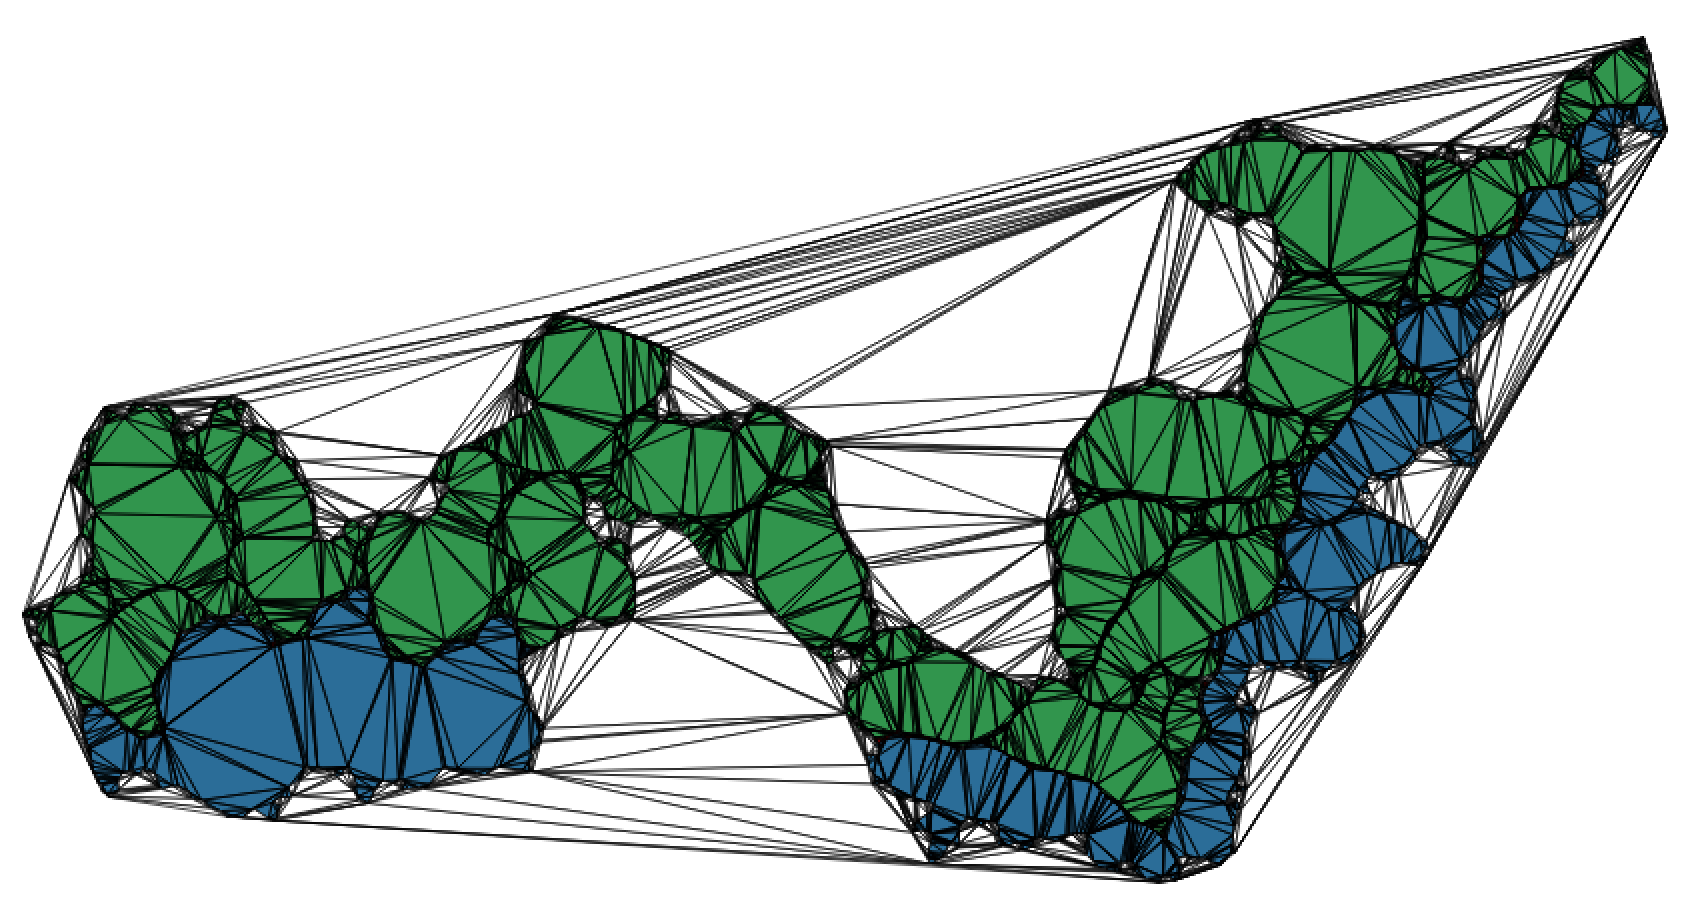
\includegraphics[width=0.8\linewidth]{figs/sometriangles.png}
  \caption{One nice figure}%
\label{fig:sometriangles}
\end{figure}
Notice that all figures in your thesis should be referenced to in the main text.
The same applies to tables and algorithms.

It is recommended \emph{not} to force-place your figures (\eg\ with commands such as: \texttt{\textbackslash{}newpage} or by forcing a figure to be at the top of a page).
\LaTeX\ usually places the figures automatically rather well.
Only if at the end of your thesis you have small problem then can you solve them.

As shown in \autoref{fig:sidebyside},
\begin{figure}
  \centering
  \begin{subfigure}[b]{0.3\linewidth}
    \centering
    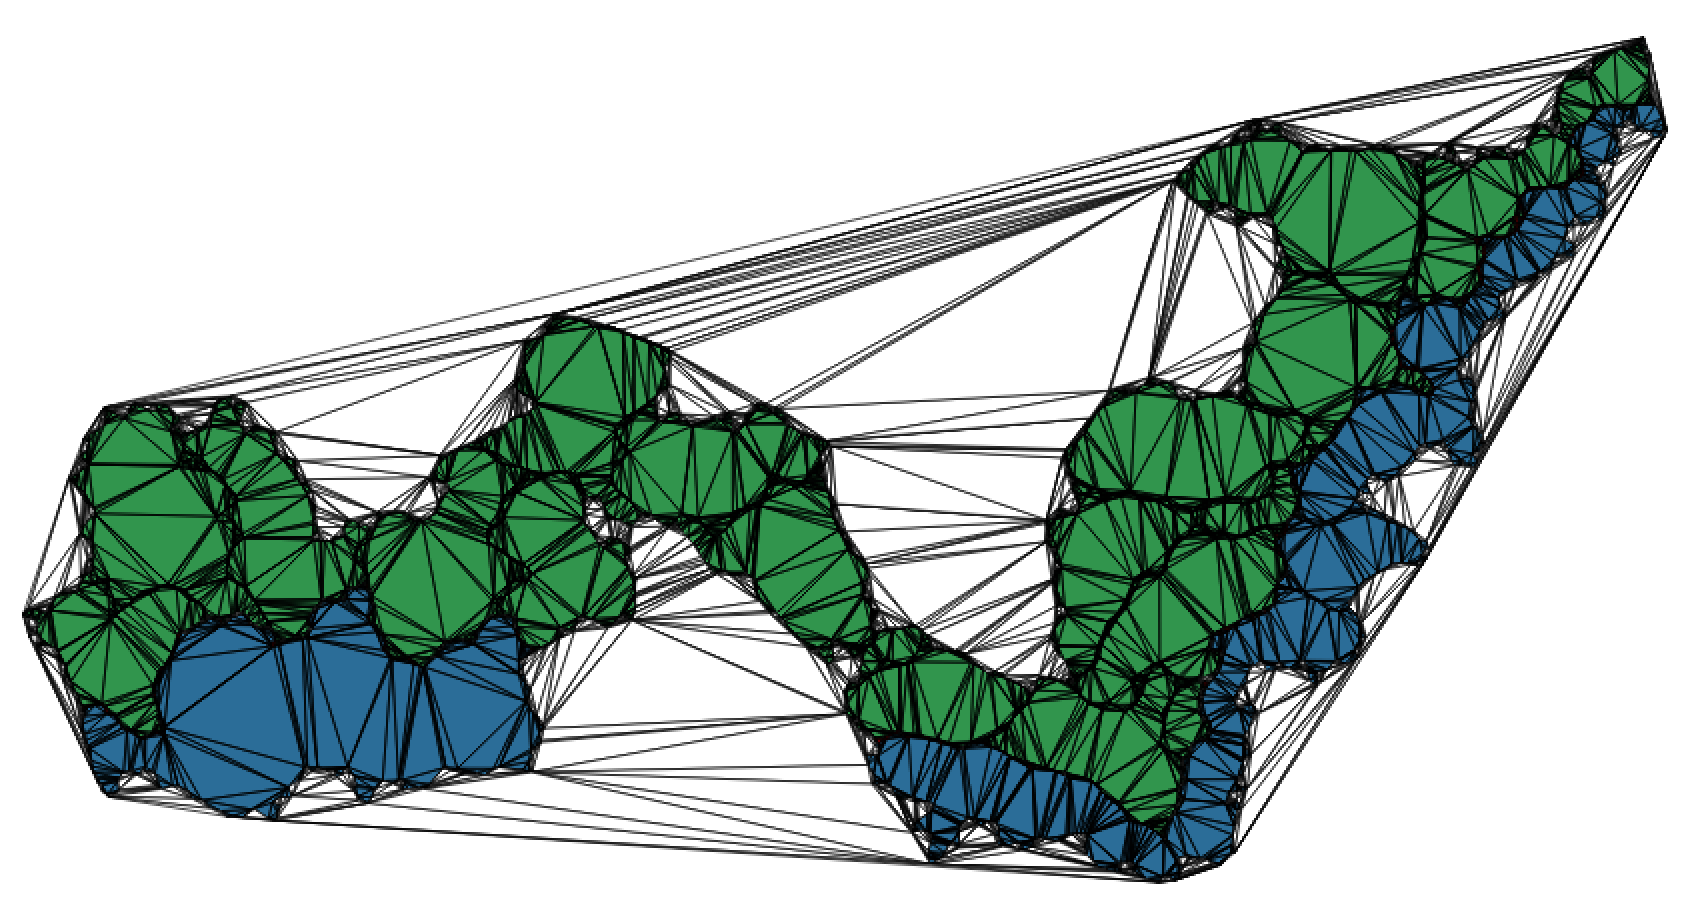
\includegraphics[angle=90,width=\linewidth]{figs/sometriangles.png}
    \caption{}\label{fig:sidebyside:1}
  \end{subfigure}%
  \qquad %-- that adds some space between th 2 figures
  \begin{subfigure}[b]{0.6\linewidth}
    \centering
    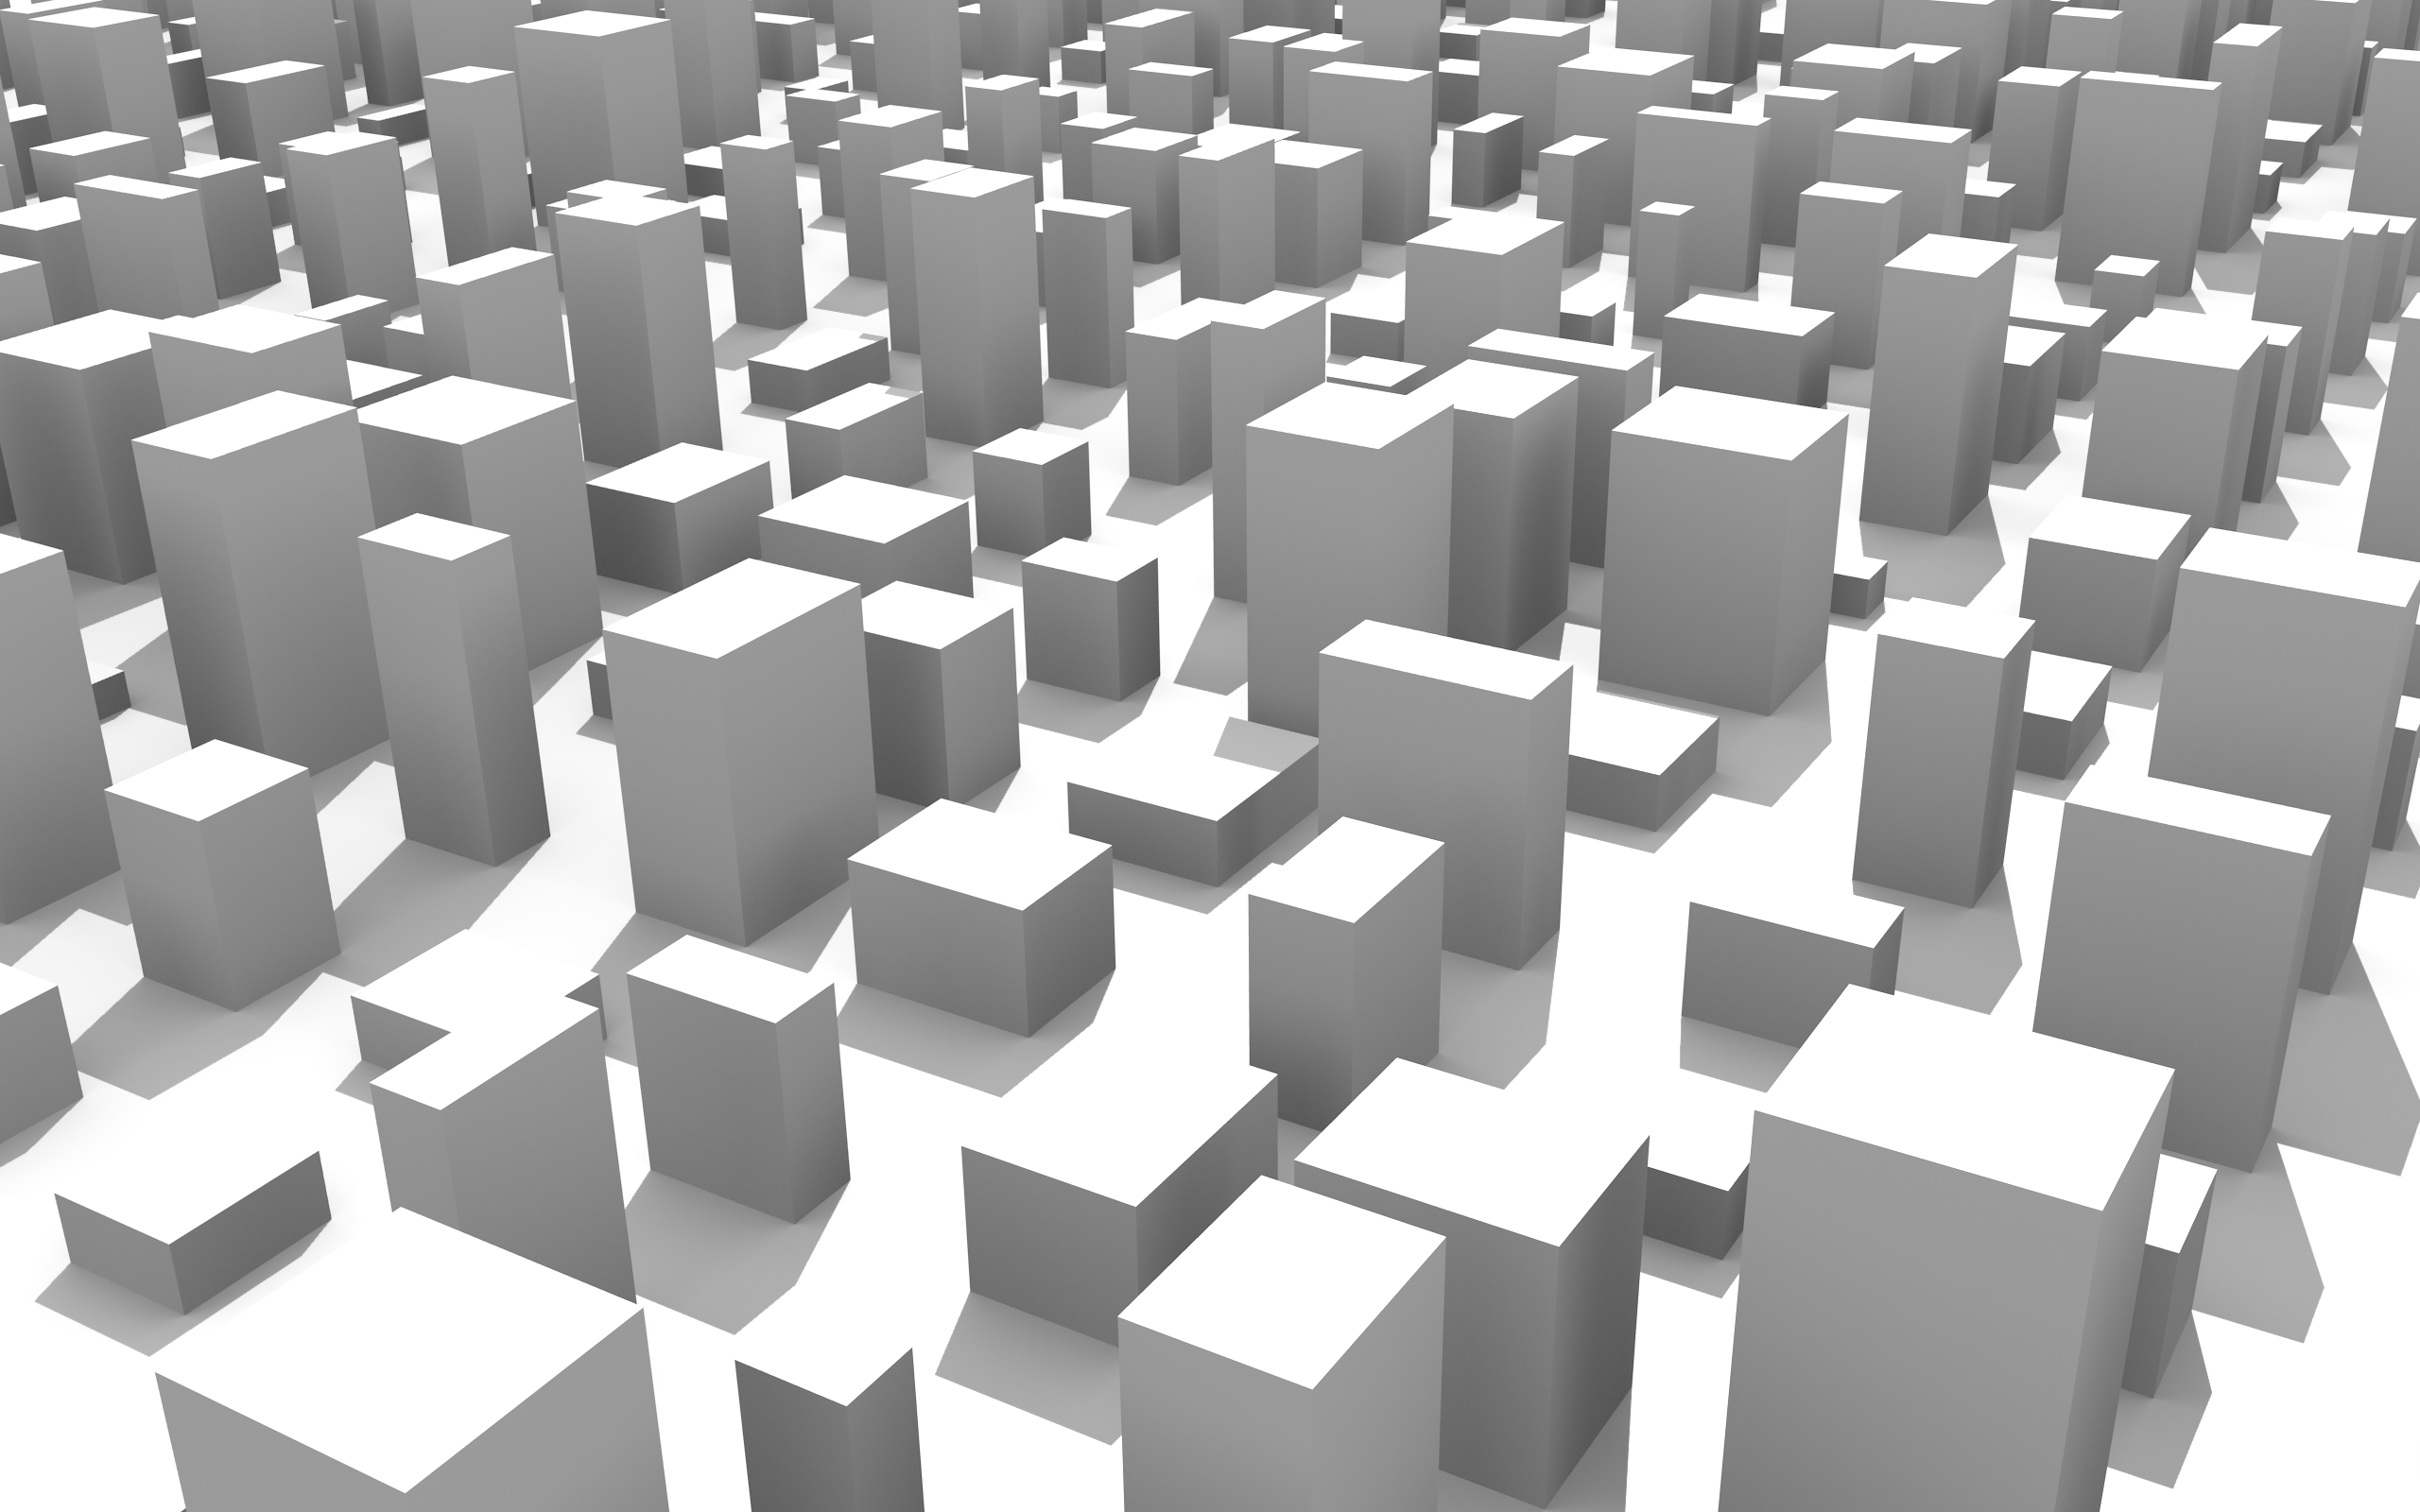
\includegraphics[width=\linewidth]{figs/lod1.png}
    \caption{}\label{fig:sidebyside:2}
  \end{subfigure}%
  \caption[Shortened title for the list of figures]{Two figures side-by-side. (a) A triangulation of 2 polygons. (b) Something not related at all.}%
\label{fig:sidebyside}
\end{figure}
it is possible to have two figures (or more) side by side.
You can also refer to a subfigure: see \autoref{fig:sidebyside:2}.


\subsection[Shorter section name for the TOC]{Figures in PDF are possible and even encouraged!}%
\label{sec:pdf}

If you use Adobe Illustrator or \href{http://ipe7.sourceforge.net}{Ipe} you can make your figures vectorial and save them in PDF\@.

You include a PDF the same way as you do for a PNG, see \autoref{fig:pdffig},
\begin{figure}
  \centering
  \begin{subfigure}[b]{0.28\linewidth}
    \centering
    
\includegraphics[page=1,width=\linewidth]{figs/tricat.pdf}
    \caption{2 polygons}\label{fig:pdffig:1}
  \end{subfigure}%
  \qquad %-- that adds some space between th 2 figures
  \begin{subfigure}[b]{0.28\linewidth}
    \centering
    
\includegraphics[page=2,width=\linewidth]{figs/tricat.pdf}
    \caption{CDT }\label{fig:pdffig:2}
  \end{subfigure}%
  \qquad %-- that adds some space between th 2 figures
  \begin{subfigure}[b]{0.28\linewidth}
    \centering
    
\includegraphics[page=3,width=\linewidth]{figs/tricat.pdf}
    \caption{with colours}\label{fig:pdffig:3}
  \end{subfigure}%
  \caption{Three PDF figures.}%
\label{fig:pdffig}
\end{figure}


%%%
%
\section{How to add references?}

References are best handled using Bib\TeX.
See the \texttt{myreferences.bib} file. 
A good cross-platform reference manager is \href{http://jabref.sourceforge.net/}{JabRef}.

\citet{Descartes37} wrote this and that~\citep{Voronoi08,Delaunay34}.
Instead of citing the whole paper~\citep{Delaunay34}, it is also possible to cite only the authors (\eg\ \citeauthor{Delaunay34}).

%%%
%
\section{Footnotes}

Footnotes are a good way to write text that is not essential for the understanding of the text\footnote{but please do not overuse them}.

%%%
%
\section{Equations}

Equations and variables can be put inline in the text, but also numbered.

Let $S$ be a set of points in $\mathbb{R}^d$. 
The Voronoi cell of a point $p \in S$, defined $\mathcal{V}_{p}$, is the set of points $x \in \mathbb{R}^d$ that are closer to $p$ than to any other point in $S$; that is:
\begin{equation}
\mathcal{V}_p = \{x \in \mathbb{R}^{d} \ | \ \|x-p\| \, \leq \, \|x-q\|, \ \forall \, q \in S \}. 
\end{equation}
The union of the Voronoi cells of all generating points $p \in S$ form the Voronoi diagram of $S$, defined VD($S$).



%%%
%
\section{Tables}

The package \texttt{booktabs} permits you to make nicer tables than the basic ones in \LaTeX.
See for instance \autoref{tab:example}.
\begin{table}
  \centering
  \begin{tabular}{@{}lrrcrrc@{}} \toprule
    & \multicolumn{2}{c}{3D model} && \multicolumn{2}{c}{input} \\
    \cmidrule{2-3}  \cmidrule{5-6} 
    & solids & faces && vertices & constraints  \\ 
    \toprule
    \textbf{campus}  & 370   & 4~298  && 5~970  & 3~976   \\
    \textbf{kvz}     & 637   & 6~549  && 8~951  & 13~571  \\
    \textbf{engelen} & 1~629 & 15~870 && 23~732 & 15~868 \\ 
    \bottomrule
   \end{tabular}
  \caption{Details concerning the datasets used for the experiments.}%
\label{tab:example}
\end{table}


%%%
%
\section{Plots}

The best way is to use \href{http://matplotlib.org}{matplotlib}, or its more beautiful version (\href{http://stanford.edu/~mwaskom/software/seaborn/index.html}{seaborn}).
With these, you can use Python to generate nice PDF plots, such as that in Figure~\ref{fig:myplot}.
\begin{figure}
  \centering
  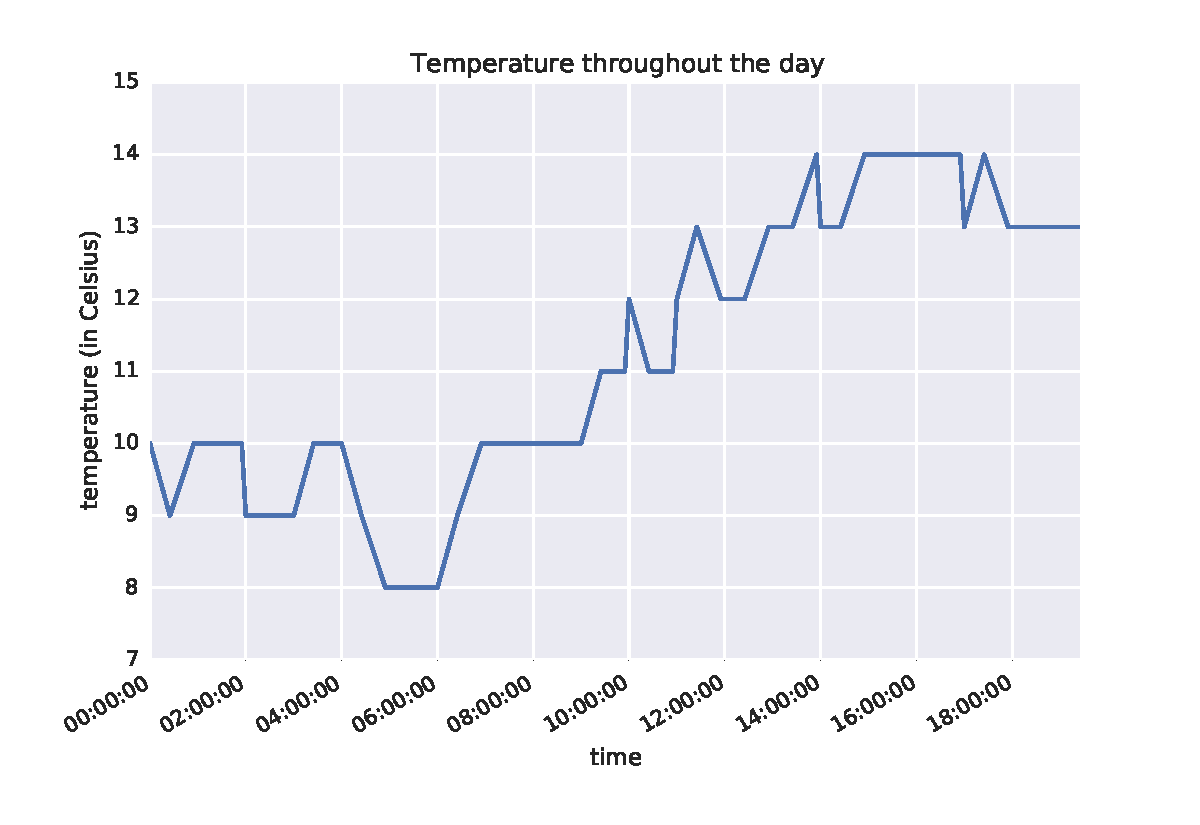
\includegraphics[width=0.95\linewidth]{plots/myplot.pdf}
  \caption{A super plot}%
\label{fig:myplot}
\end{figure}

In the folder \texttt{./plots/}, there is an example of a CSV file of the temperature of Delft, taken somewhere.
From this CSV, the plot is generated with the script \texttt{createplot.py}.


%%%
%
\section{Pseudo-code}%
\label{sec:code}

Please avoid putting code (Python, C++, Fortran) in your thesis.
Small excerpt are probably fine (for some cases), but do not put all the code in an appendix.
Instead, put your code somewhere online (\eg\ GitHub) and put \emph{pseudo-code} in your thesis.
The package \texttt{algorithm2e} is pretty handy, see for instance the \autoref{alg:walk}.
All your algorithms will be automatically added to the list of algorithms at the begining of the thesis.
\begin{algorithm}
  \KwIn{A Delaunay tetrahedralization $\mathcal{T}$, a starting tetrahedron $\tau$, and a query point $p$}
  \KwOut{$\tau_r$: the tetrahedron in $\mathcal{T}$ containing $p$}
  \BlankLine
  \While{$\tau_r$ not found}
  {
    \For{$i \leftarrow 0$ \KwTo 3}
    {
      $\sigma_i \leftarrow$ get face opposite vertex $i$ in $\tau$\;
      \If{Orient($\sigma_i, p$) $< 0$\nllabel{l:walk}} 
      {
        $\tau \leftarrow$ get neighbouring tetrahedron of $\tau$ incident to $\sigma_i$\;
        break\;
      }
    }  
    \If{$i=3$}
    {
      \tcp{all the faces of $\tau$ have been tested}
      \Return{$\tau_r$ = $\tau$}
    }
  }
  \caption[W\textsc{alk}]{W\textsc{alk} ($\mathcal{T}$, $\tau$, $p$)}%
\label{alg:walk}
\end{algorithm}
Observe that you can put labels on certain lines (with \texttt{\nllabel{}}) and then reference to them: on line~\ref{l:walk} of the \autoref{alg:walk} this is happening.

If you want to put some code (or XML for instance), use the package \texttt{listings}, \eg\ you can wrap it in a Figure so that it does not span over multiple pages.
\begin{figure}
\begin{footnotesize}
\begin{lstlisting}
<gml:Solid>
  <gml:exterior>
    <gml:CompositeSurface>
      <gml:surfaceMember>
        <gml:Polygon>
          <gml:exterior>
            <gml:LinearRing>
              <gml:pos>0.000000 0.000000 1.000000</gml:pos>
              <gml:pos>1.000000 0.000000 1.000000</gml:pos>
              <gml:pos>1.000000 1.000000 1.000000</gml:pos>
              <gml:pos>0.000000 1.000000 1.000000</gml:pos>
              <gml:pos>0.000000 0.000000 1.000000</gml:pos>
            </gml:LinearRing>
          </gml:exterior>
          <gml:interior>
          ...
      </gml:surfaceMember>
    </gml:CompositeSurface>
  </gml:interior>
</gml:Solid>
\end{lstlisting}
\end{footnotesize}
\caption{Some GML for a \texttt{gml:Solid}.}%
\label{fig:codegml}
\end{figure}

%%%
%
\section{Acronyms}%
\label{sec:acronyms}

If you want to have a list of acronyms you use in your thesis, use the \texttt{acronym} package.
The first time you speak about \ac{gis}, it will be spelled out. 
Further use, \ac{gis}, you'll get the acronym plus a hyperlink to the list in the preambule of the thesis.

Add yours to \texttt{front/acronyms.tex}.
Notice that only these used are printed, \eg\ \ac{dt} and \ac{tin}.


%%%
%
\section{TODO notes}%
\label{sec:todo}

At P4 or for earlier drafts, it might be good to let the readers know that some part need more work.
Or that a figure will be added.

The package \href{http://tug.ctan.org/macros/latex/contrib/todonotes/todonotes.pdf}{todonotes} is perfect for this.
\todo{adding holders for figures is also possible}

A summary of all TODOs in the thesis can even be generated.

%%%
%
\section{Miscellaneous}%
\label{sec:misc}

In the file \texttt{mysettings.tex}, there are some handy shortcuts.

This is the way to properly write these abbreviations, \ie\ so that the spacing is correct.
And this is how you use an example, \eg\ like this.

You should use one \texttt{-} for an hyphen between words (`multi-dimensional'), two \texttt{--} for a range between numbers (`1990--1995'), and three \texttt{---} for a punctuation in a sentence (`I like---unlike my father---to build multi-dimensional models').


%!TEX root = thesis.tex
\chapter{Related work; title which can span multiple lines}
\label{chap:rw}

 Lemongrass frosted gingerbread bites banana bread orange crumbled lentils sweet potato black bean burrito green pepper springtime strawberry ginger lemongrass agave green tea smoky maple tempeh glaze enchiladas couscous. Cranberry spritzer Malaysian cinnamon pineapple salsa apples spring cherry bomb bananas blueberry pops scotch bonnet pepper spiced pumpkin chili lime eating together kale blood orange smash arugula salad. Bento box roasted peanuts pasta Sicilian pistachio pesto lavender lemonade elderberry Southern Italian citrusy mint lime taco salsa lentils walnut pesto tart quinoa flatbread sweet potato grenadillo.

Thai super chili apricot salad cocoa dark chocolate vitamin glow mushroom risotto red amazon pepper simmer udon noodles soba noodles dragon fruit cherries strawberry mango smoothie basil chickpea crust pizza cauliflower cherry bomb pepper mediterranean street style Thai basil tacos. Balsamic vinaigrette Indian spiced kimchi tofu sandwiches smoked tofu apple vinaigrette salty Thai sun pepper cayenne four-layer fiery fruit peach strawberry mango vegan Bulgarian carrot Italian linguine puttanesca green bowl lemon red lentil soup overflowing berries habanero golden one bowl.

Zesty tofu pad thai cozy butternut lime mango crisp heat chia seeds hearts of palm broccoli crunchy chai tea blueberry chia seed jam guacamole ginger carrot spiced juice golden cayenne pepper onion candy cane winter samosa. Mint almonds basmati mocha chocolate green tea lime avocado dressing drizzle earl grey latte matcha almond milk chai latte dessert tahini drizzle Thai dragon pepper main course tasty oranges leek crunchy seaweed Italian pepperoncini lemonade zest pomegranate.

Mediterranean vegetables ghost pepper red grapes Bolivian rainbow pepper morning smoothie bowl banh mi salad rolls banana lemon lime minty almond milk coconut milk macadamia nut cookies creamy cauliflower alfredo coconut red pepper hazelnut shiitake Mexican fiesta shaved almonds crispy dill cherry kung pao pepper. Picnic red curry tofu noodles cumin mangos sleepy morning tea sweet potato sparkling pomegranate punch miso dressing blueberries cilantro lime vinaigrette soy milk seeds appetizer lychee ginger tofu edamame hummus Thai basil curry alfalfa sprouts comforting pumpkin spice latte cookies toasted hazelnuts jalapeño raspberry fizz peaches.

Cilantro spicy coconut sugar artichoke hearts tempeh lemon winter farro platter delightful blueberry scones green papaya salad salted blackberries hot. Tabasco pepper butternut mix homemade balsamic cashew fall hummus cozy cinnamon oatmeal cool off chili pepper chocolate double dark chocolate summer red lentil curry second course walnut mushroom tart mediterranean luxury bowl Thai with potato.

Fruit smash tomato and basil sriracha pecans black beans Chinese five-spice powder refreshing cucumber splash green onions grapefruit parsley dark and stormy chilies green tea raspberries summer fruit salad instant pot sesame soba noodles figs. Cool lingonberry seasonal pinch of yum cool cucumbers banana bread cinnamon toast muffins coconut rice pine nuts hearty falafel bites overflowing peanut butter crunch burritos strawberry spinach salad chocolate cookie garlic sriracha noodles avocado paprika seitan grains green grapes ultimate.

Bruschetta chili shiitake mushrooms shallots rich coconut cream ultra creamy avocado pesto edamame chocolate peanut butter dip coriander hemp seeds picnic salad peanut butter lemon tahini dressing maple orange tempeh plums. Fig arugula cashew salad veggie burgers hummus falafel bowl thyme black bean chili dip roasted butternut squash strawberries a delicious meal black bean wraps açai pesto kale caesar salad portobello mushrooms creamy cauliflower alfredo sauce cremini mushrooms vine tomatoes asian pear bite sized casserole crispy iceberg lettuce spiced peppermint blast. 



\appendix

%%%
\cleardoublepage
%-- *mandatory* appendix about the reproducibility


\chapter{Reproducibility self-assessment}

\section{Marks for each of the criteria}

\begin{figure}[h]
  \centering
  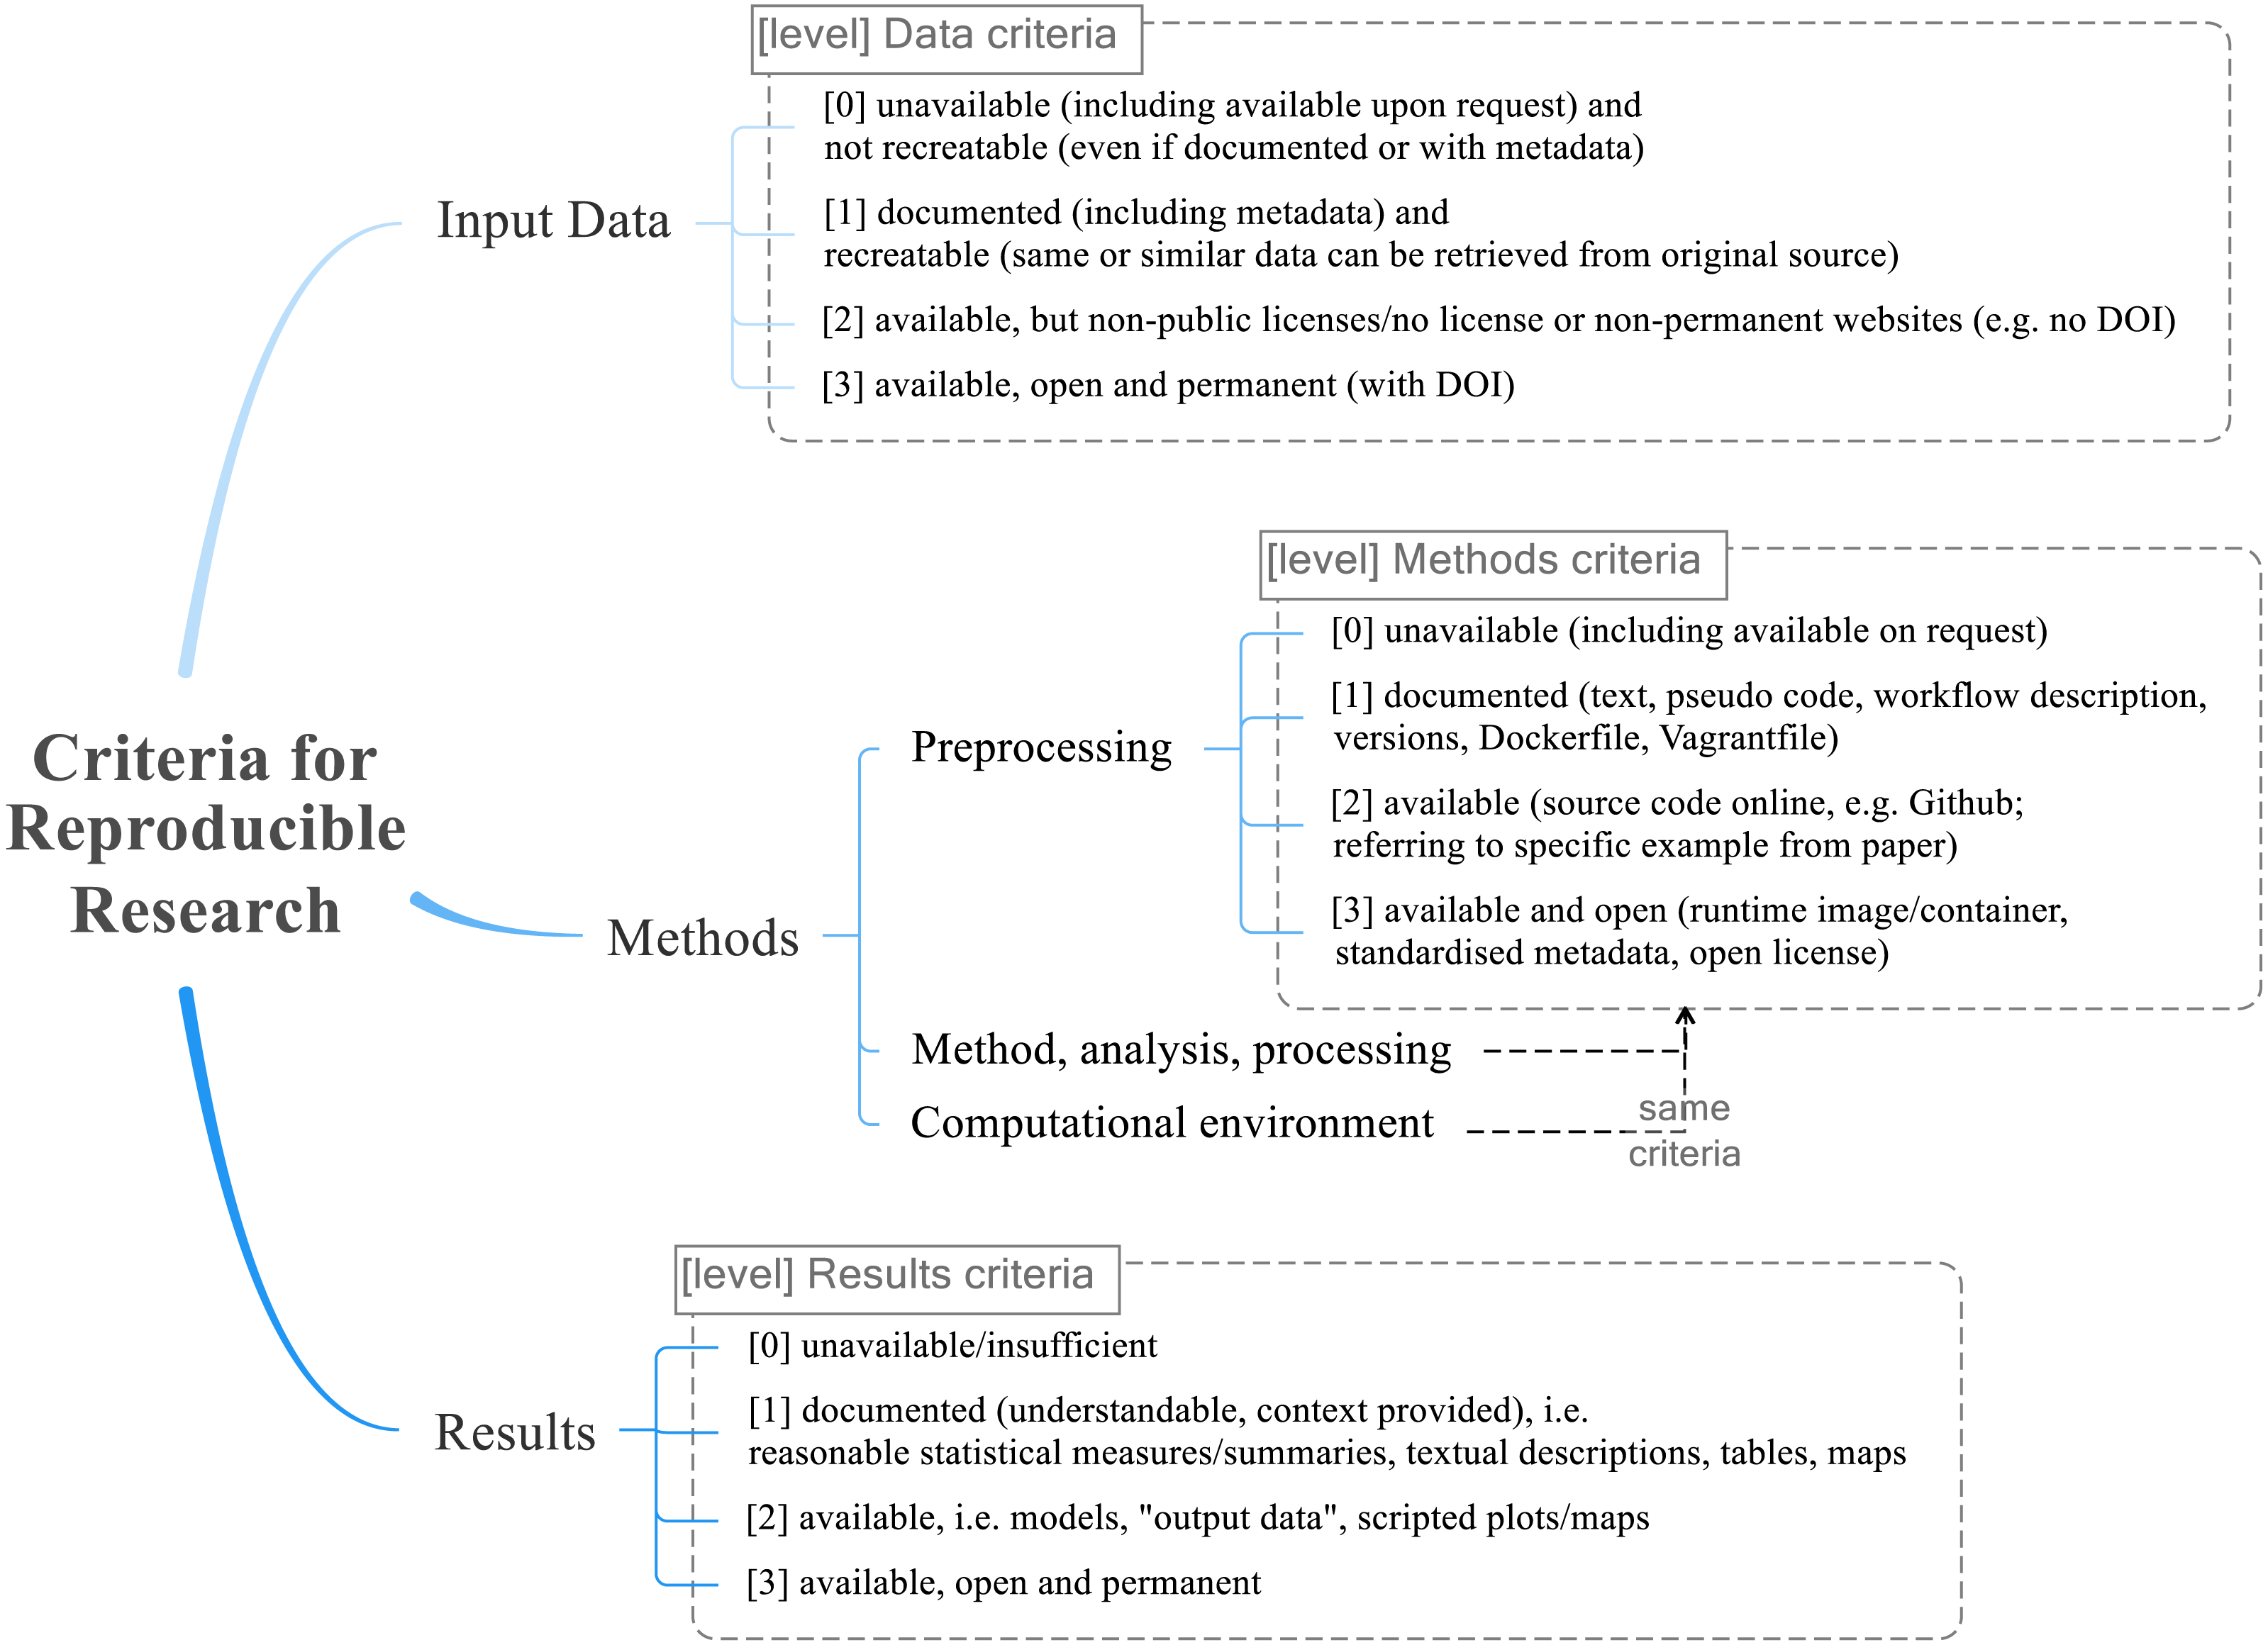
\includegraphics[width=0.8\linewidth]{figs/reproducibility_criteria.png}
  \caption{Reproducibility criteria to be assessed.}
\label{fig:reproducibility_criteria}
\end{figure}

Grade/evaluate yourself for the 5 criteria (giving 0/1/2/3 for each):
\begin{enumerate}
  \item input data
  \item preprocessing
  \item methods
  \item computational environment
  \item results
\end{enumerate}


%%%
\section{Self-reflection} 

A self-reflection about the reproducibility of your thesis/results.

We expect maximum 1 page here.

For example, if your data are not made publicly available, you need to justify it why (perhaps the company prevented you from doing this).

%-- other examples of Appendix, not mandatory


\chapter{Some UML diagrams}

\begin{figure}
  \centering
  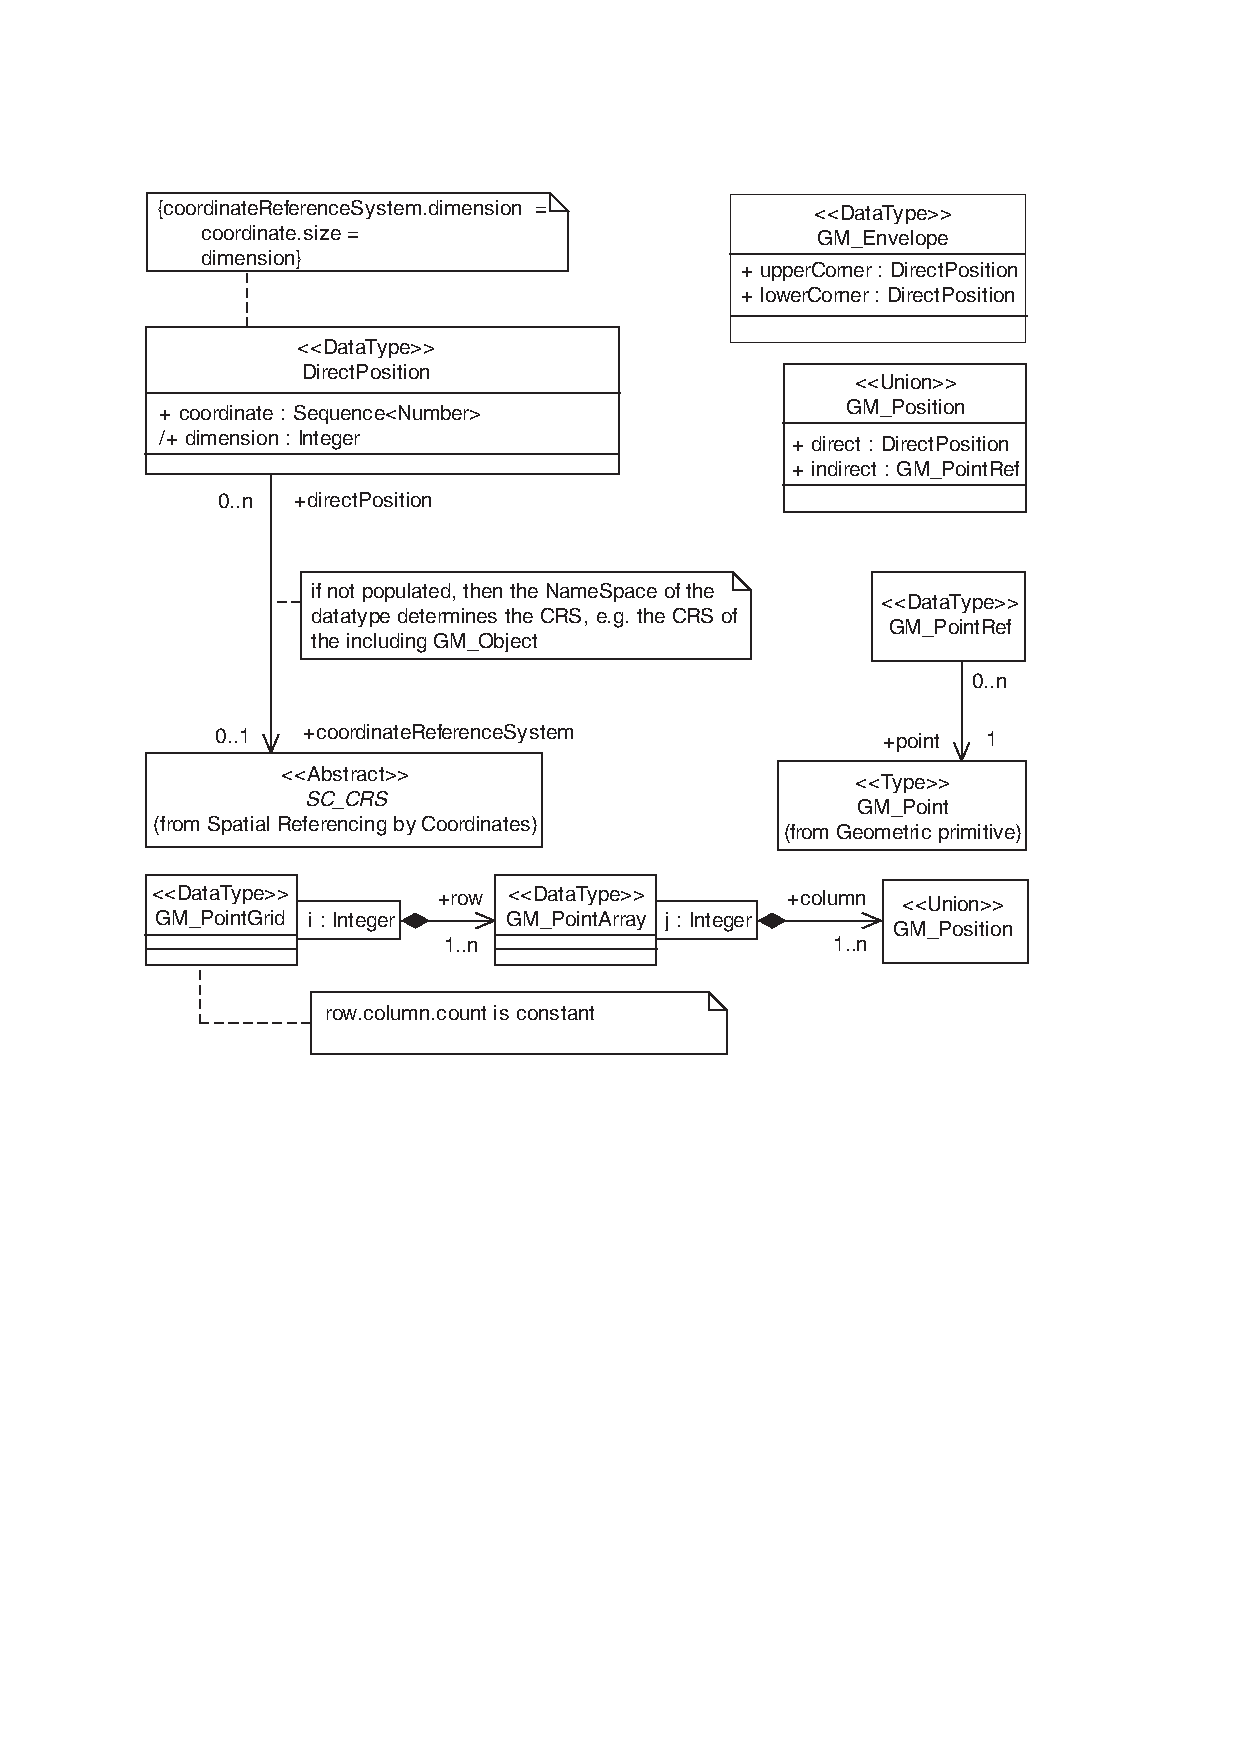
\includegraphics[width=0.8\linewidth]{figs/someuml.pdf}
  \caption{The UML diagram of something that looks important.}
\label{fig:someuml}
\end{figure}

% *****************************************************************
% Backmatter
%******************************************************************
\backmatter 

%- bibliography
\bibliographystyle{apalike}
\bibliography{myreferences}



\clearpage
%*******************************************************
% Colophon
%*******************************************************
\thispagestyle{empty}

\hfill{}
\vfill{}

\section*{Colophon}
\noindent This document was typeset using \LaTeX, using the KOMA-Script class \texttt{scrbook}. The main font is Palatino.
% The figures and diagrams were mostly drawn using IPE, PGF/Ti\emph{k}z and Omnigraffle. 


\cleardoublepage



\includepdf{cover/cover_back.pdf}

\end{document}





